% Dual-layer resist stack showing undercut for clean lift-off
\begin{figure}[htbp]
  \centering
  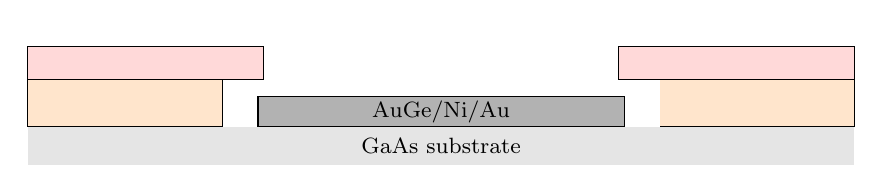
\begin{tikzpicture}[x=1.5cm,y=0.6cm,font=\footnotesize]
    % Dimensions
    \def\w{7}
    \def\hsub{0.8}
    \def\hlor{1.0}
    \def\hs1803{0.7}
    \def\gap{0.35}
    \def\xL{2.0}
    \def\xR{5.0}

    % Keep bounding box tight to the main drawing so labels don't shift centering
    \path[use as bounding box] (0,0) rectangle (\w,\hsub+\hlor+\hs1803+0.4);

    % Substrate (GaAs)
    \fill[gray!20] (0,0) rectangle (\w,\hsub);
    \node at (3.5,0.4) {GaAs substrate};

    % LOR with wider opening (split to avoid outlines across the gap)
    \fill[orange!20] (0,\hsub) rectangle (\xL-\gap,\hsub+\hlor);
    \draw (0,\hsub) rectangle (\xL-\gap,\hsub+\hlor);
    \fill[orange!20] (\xR+\gap,\hsub) rectangle (\w,\hsub+\hlor);
    \draw (\xR+\gap,\hsub) rectangle (\w,\hsub+\hlor);

    % Remove opening in LOR (undercut wider)
    \fill[white] (\xL-\gap,\hsub) rectangle (\xR+\gap,\hsub+\hlor);
    \node[anchor=east] at (-0.2,\hsub+0.5*\hlor) {LOR (undercut)};

    % S1803 with narrower opening (split to avoid outlines across the gap)
    \fill[red!15] (0,\hsub+\hlor) rectangle (\xL,\hsub+\hlor+\hs1803);
    \draw (0,\hsub+\hlor) rectangle (\xL,\hsub+\hlor+\hs1803);
    \fill[red!15] (\xR,\hsub+\hlor) rectangle (\w,\hsub+\hlor+\hs1803);
    \draw (\xR,\hsub+\hlor) rectangle (\w,\hsub+\hlor+\hs1803);
    \fill[white] (\xL,\hsub+\hlor) rectangle (\xR,\hsub+\hlor+\hs1803);
    \node[anchor=east] at (-0.2,\hsub+\hlor+0.5*\hs1803) {S1803};

    % Metal deposition (wider, under the S1803 opening)
    \fill[gray!60] (\xL-0.05,\hsub) rectangle (\xR+0.05,\hsub+0.65);
    \draw (\xL+-0.05,\hsub) rectangle (\xR+0.05,\hsub+0.65);
    \node at (3.5,\hsub+0.32) {AuGe/Ni/Au};

  \end{tikzpicture}
  \caption{Dual-layer LOR/S1803 resist stack after development showing the wider LOR opening that creates an undercut for clean metal lift-off.}
  \label{fig:lift_off_stack}
\end{figure}
